% EE2000 Final Project Report -- Fall 2026, IIT Hyderabad
% Topic: Real-Time Multichannel EEG Seizure Detection on FPGA (DWT + Linear SVM)
% Template: IEEE/CVF (cvpr.sty review format)
% Note: All content added for the Final Report milestone is strictly marked in blue text.
% Team: 15

\documentclass[10pt,twocolumn,letterpaper]{article}

\usepackage[review]{cvpr} 
\usepackage{graphicx}
\graphicspath{{../results/}{results/}}
\usepackage{amsmath}
\usepackage{amssymb}
\usepackage{booktabs}
\usepackage{tabularx}
\usepackage{tikz}
\usetikzlibrary{arrows.meta,positioning,fit,backgrounds}
\usepackage[dvipsnames]{xcolor}

\usepackage[pagebackref,breaklinks,colorlinks,allcolors=cvprblue]{hyperref}
\def\paperID{15}
\def\confName{EE2000}
\def\confYear{2026}

\title{Real-Time Multichannel EEG Seizure Detection on FPGA Using Discrete Wavelet Transform and Linear Support Vector Machine: Final Project Report}

\author{EE2000 Project Team 15\\[2pt]
Department of Electrical Engineering, Indian Institute of Technology Hyderabad}
\definecolor{cvprblue}{rgb}{0.21,0.49,0.74}
\setlength{\bibsep}{0.0pt}

\renewcommand{\topfraction}{0.95}
\renewcommand{\bottomfraction}{0.95}
\renewcommand{\textfraction}{0.05}
\renewcommand{\floatpagefraction}{0.85}

\begin{document}
\maketitle

%---------------------------------------------------------------------
\begin{abstract}
Automatic detection of epileptic seizures from scalp electroencephalography (EEG) is a nonstationary, heavily class-imbalanced signal-processing problem in which detection sensitivity, false alarms, and latency must be balanced under stringent embedded resource constraints. This report presents a complete, real-time streaming seizure-detection pipeline implemented on the RealDigital Boolean Board (AMD Spartan-7 XC7S50 FPGA). The system band-limits 22 bipolar EEG channels with a 4th-order causal Butterworth IIR filter (0.5--25\,Hz, realized as two cascaded Second-Order Sections), computes a 5-level Daubechies-4 discrete wavelet transform (DWT), accumulates sub-band Energy and Line-Length features across 2.0\,s sliding windows (1.0\,s hop), and classifies windows using a Linear Support Vector Machine (SVM) whose normalization parameters and weights are algebraically folded offline. A temporal post-processing FSM asserts an alarm after $k=3$ consecutive positive windows with a 30\,s refractory blanking period.

Evaluated on the CHB-MIT Scalp EEG Database across 47 recordings from subjects \texttt{chb01}, \texttt{chb02}, and \texttt{chb03} (17 clinical seizures, 45.63 total non-ictal evaluation hours; 165,237 total windows) under a strict Leave-One-Record-Out (LORO) protocol, our pipeline achieves \textbf{100.0\% sensitivity} (17/17 seizures detected; exact 95\% Clopper-Pearson CI: $[80.5\%, 100.0\%]$), \textbf{0.373 false alarms per hour} ($\approx 1$ false alarm every 2.68\,h), and a median detection latency of \textbf{3.0\,s}. Independent replication of the benchmark Shoeb \& Guttag (2010) filter-bank RBF-SVM baseline on our identical partition achieves 88.2\% sensitivity and 0.307\,FA/h ($p \approx 0.50$ McNemar test; overlapping Poisson 95\% CIs), while our linear architecture provides an empirical 2.0\,s faster median detection latency (3.0\,s vs.\ 5.0\,s) while eliminating non-linear kernel evaluations against high-dimensional support vectors in $\mathbb{R}^{528}$ (whose count is substantially inflated under untuned default hyperparameters) via a single 176-multiply dot product.

A full-cohort fixed-point re-evaluation under 16-bit Q1.15 arithmetic demonstrates zero event-level metric degradation ($\Delta = 0.0\%$ sensitivity and FA/h parity) with 82.6\,dB SQNR. The complete synthesizable Verilog RTL datapath closes timing at 100\,MHz on the Spartan-7 XC7S50 with positive slack ($WNS = +1.842$\,ns, $WHS = +0.128$\,ns), utilizing only 1,418 Slice LUTs (4.35\%), 1,784 Slice Registers (2.74\%), 2 DSP48E1 slices (1.67\%), and 2 Block RAMs (1.33\%), dissipating 118\,mW total on-chip power. Real-time playback over a 230,400-baud UART stream confirms physical alarm assertion on board LEDs, RGB status indicators, and an 8-digit multiplexed 7-segment display, with cycle-accurate testbenches validating the causal filter group delay ($d_{\text{DWT}} \approx 0.25$\,s).

\medskip
\noindent\textbf{Keywords:} EEG seizure detection, discrete wavelet transform (DWT), linear SVM, offline weight folding, dynamic wire-shifting, Spartan-7 FPGA, RealDigital Boolean Board, fixed-point arithmetic.

{\color{blue}
\medskip
\noindent\textbf{Final Project Milestone Update:}
This final report builds directly upon our preliminary proposal and mid-term report. The preliminary phase established the theoretical formulation and Boolean Board target. The mid-term milestone established the frozen 47-recording CHB-MIT benchmark, the Python floating-point LORO baseline (100.0\% sensitivity, 0.373\,FA/h), the Shoeb \& Guttag (2010) replication, and 4D ablation studies. This final submission delivers the complete physical realization: synthesizable Verilog RTL datapath, Vivado 100\,MHz timing closure on the Spartan-7 XC7S50, physical 230,400-baud UART streaming demonstration with board peripherals, and decision-level full-cohort fixed-point verification ($\Delta = 0.0\%$).
}
\end{abstract}

%---------------------------------------------------------------------
\section{Introduction}
\label{sec:intro}

Scalp EEG records the summed electrical activity of large neuronal populations as microvolt-level voltage differences between electrodes. Seizure activity typically appears as rhythmic, multi-component activity whose spectral content, spatial distribution, and time course differ between patients and even between seizures of the same patient \cite{shoeb2010icml}. Detecting seizure onset automatically is therefore a signal-processing problem before it is a clinical one: a detector must separate seizure activity from normal background rhythms, sleep spindles, and artifacts, using short segments of a noisy, multi-channel, nonstationary signal.

Four properties make the problem difficult. First, EEG is nonstationary: its statistics change within and between the seizure and non-seizure states, and a single seizure can evolve in amplitude and frequency over a few seconds \cite{shoeb2010icml}. Second, the signal is noisy and contaminated by non-cerebral artifacts (ocular, muscular, and electrode motion). Third, seizure-related events are transient, so a detector must react to short-lived patterns without introducing intolerable false alarms. Fourth, there is strong inter-patient variability: EEG that indicates a seizure in one patient can resemble a benign pattern in another \cite{shoeb2010icml}. These properties motivate time--frequency analysis rather than a single global spectrum.

The discrete wavelet transform (DWT) is a natural candidate. It decomposes a signal with a multiresolution filter bank, giving coarse-to-fine sub-bands with time localisation \cite{mallat1989theory}. The Daubechies family of compactly supported orthonormal wavelets \cite{daubechies1988orthonormal} appears widely in the EEG literature, including the db4 wavelet \cite{shen2022dwt,subasi2007eeg}. Statistics of the wavelet coefficients (such as energy and line-length per sub-band) can then be passed to a classifier such as a support vector machine (SVM) \cite{cortes1995support}.

\paragraph{Why implement this on an FPGA?} An FPGA is not required strictly for raw throughput at 256\,Hz: as Sec.~\ref{sec:fpga} shows, the arithmetic load is modest and a conventional microcontroller could execute the sequential arithmetic. The primary engineering motivation is cycle-accurate determinism, hardware--software co-design, and fixed-point verification. The pipeline is a regular, multiply--accumulate-dominated streaming design, making the FPGA an ideal testbed for word-length profiling, zero-jitter latency, dynamic-range optimization, and cycle-accurate verification against a software reference model.

\paragraph{Target platform.} The Boolean Board is an educational development platform built around an AMD Spartan-7 XC7S50 FPGA (\texttt{xc7s50csga324-1}) \cite{realdigital2024boolean}. The device provides 120 DSP48E1 slices, 75 36-Kb Block RAMs (or 150 18-Kb primitives), 32,600 logic LUTs, and 65,200 flip-flops. The board features an on-board CP2102N USB-UART bridge, 16 user LEDs, 16 slide switches, two RGB LEDs, and an eight-digit multiplexed seven-segment display. These peripherals provide complete infrastructure for real-time dataset playback and immediate visual alarm validation.

\paragraph{Contribution and scope.} This project realizes a complete, verified, and physically demonstrated engineering pipeline. We do not claim algorithmic novelty; rather, the contribution lies in:
\begin{enumerate}
    \item A fully frozen, reproducible software baseline implementing causal IIR filtering, 5-level db4 DWT, and linear SVM under strict patient-specific Leave-One-Record-Out (LORO) cross-validation across 47 CHB-MIT recordings.
    \item An independent benchmark replication of the foundational Shoeb \& Guttag \cite{shoeb2010icml} filter-bank RBF-SVM baseline on our identical cohort partition.
    \item A thorough 4-dimension ablation study ($k$-persistence, feature sets, sub-band pruning, regularization) and finite word-length analysis ($B \in [8, 16]$ bits).
    \item Full-cohort fixed-point re-evaluation demonstrating exact $100.0\%$ sensitivity and 0.373\,FA/h parity ($\Delta = 0.0\%$).
    \item A fully synthesizable Verilog RTL datapath incorporating offline algebraic weight folding and dynamic-range wire-shifting, closing timing at 100\,MHz on the Spartan-7 XC7S50 while consuming $<5\%$ logic resources and 118\,mW power.
    \item Physical verification via 230,400-baud UART playback demonstrating real-time alarm assertions on Boolean Board LEDs and 7-segment displays.
\end{enumerate}

{\color{blue}
\paragraph{Progression from Preliminary and Mid-Term Reports.}
This report documents the cumulative three-stage evolution of Team 15's project:
\begin{itemize}
    \item \textbf{Preliminary Proposal:} Formulated the clinical problem, established the mathematical foundation of dyadic DWT + SVM, and selected the AMD Spartan-7 XC7S50 (RealDigital Boolean Board) architecture.
    \item \textbf{Mid-Term Milestone:} Froze the 47-recording CHB-MIT cohort (17 seizures, 45.63 control hours), validated the software streaming baseline under patient-specific LORO cross-validation, replicated the Shoeb \& Guttag (2010) benchmark, and completed 4D ablation studies.
    \item \textbf{Final Endsem Milestone (This Work):} Implemented the complete synthesizable Verilog RTL datapath (IIR biquads, 5-level db4 DWT, dynamic-range wire-shifting, folded linear SVM), achieved 100\,MHz Vivado timing closure, conducted full-cohort fixed-point LORO re-evaluation, and physically demonstrated real-time seizure alarms via 230,400-baud UART on the Boolean Board.
\end{itemize}
}

\subsection{Problem Statement}
\label{sec:problem}

The objective is to design, implement, and evaluate a real-time FPGA-based EEG seizure-detection processor. Formally, for datapath word length $B$ and pipeline parameters $\theta$, we frame this as a hardware-constrained optimization problem:
\begin{equation}
\begin{aligned}
\max_{\theta,B}\;& \mathrm{Sens}(\theta,B)\\
\text{s.t.}\;& \mathrm{FA/h}(\theta,B)\le\epsilon,\quad L(\theta,B)\le\tau,\\
& N_{\mathrm{DSP}}(B)\le 120,\quad M_{\mathrm{BRAM}}(B)\le 150,
\end{aligned}
\label{eq:problem}
\end{equation}
where $\mathrm{Sens}$ is event sensitivity, $\mathrm{FA/h}$ is false-alarm rate, $L$ is median detection latency, and $N_{\mathrm{DSP}}$ and $M_{\mathrm{BRAM}}$ are DSP48E1 and 18-Kb BRAM utilization. In our implementation, SVM weights are trained offline via regularized hinge-loss minimization, while $B$ and post-processing parameter $k$ are swept. We adopt clinical targets of $\epsilon \le 0.50\,\text{h}^{-1}$ and detection delay $\tau \le 5.0$\,s, both of which are satisfied by our streaming processor on the pooled evaluation cohort (0.373\,FA/h, 3.0\,s median latency; per-subject breakdown discussed in Sec.~\ref{sec:proposed_results}).

%---------------------------------------------------------------------
\section{Clinical Context and Dataset}
\label{sec:dataset}

The primary benchmark is the CHB-MIT Scalp EEG Database hosted by PhysioNet \cite{guttag2010chbmit,goldberger2000physionet}, collected at Boston Children's Hospital and introduced in the seminal work of Shoeb and colleagues \cite{shoeb2009thesis,shoeb2010icml}:
\begin{itemize}
  \item The database contains continuous EEG from pediatric subjects with intractable epilepsy. Recordings are grouped into 23 original pediatric cases (22 subjects, with \texttt{chb21} recorded 1.5 years after \texttt{chb01} from the same subject); adult case \texttt{chb24} was added in 2010, totaling 24 cases.
  \item Signals were sampled at 256 samples/s with 16-bit resolution using the international 10--20 electrode placement.
  \item The collection comprises 664 \texttt{.edf} files (42.6\,GB), of which 129 contain one or more annotated seizures (198 total seizures). Files typically span 1.0 hour.
\end{itemize}

Channel layout across cases is non-uniform: most records hold 23 bipolar channels, but auxiliary signals (ECG in \texttt{chb04}, vagal-nerve-stimulator signals in \texttt{chb09}) or dummy channels (``-'') appear in certain records.

\subsection{Frozen Dataset Selection and Channel Harmonization}
\label{sec:dataset_selection}

To eliminate data-selection bias, we applied a strict mechanical selection rule to all 24 cases in CHB-MIT prior to evaluating classifiers:
\begin{enumerate}
    \item Select the first three eligible cases in numerical order with at least 3 annotated seizures.
    \item Require a consistent 23-channel bipolar montage without non-cerebral auxiliary channels (e.g., ECG or VNS).
    \item Treat \texttt{chb01} and \texttt{chb21} as a single patient cohort (with \texttt{chb21} set aside to preserve subject-level partition independence).
\end{enumerate}

Cases \texttt{chb01}, \texttt{chb02}, and \texttt{chb03} passed all criteria. Header parsing revealed that channel 15 and channel 23 both record \texttt{T8-P8}. Discarding the duplicate entry yielded 22 unique bipolar channels consistently present across all recordings:
\texttt{FP1-F7}, \texttt{F7-T7}, \texttt{T7-P7}, \texttt{P7-O1}, \texttt{FP1-F3}, \texttt{F3-C3}, \texttt{C3-P3}, \texttt{P3-O1}, \texttt{FP2-F4}, \texttt{F4-C4}, \texttt{C4-P4}, \texttt{P4-O2}, \texttt{FP2-F8}, \texttt{F8-T8}, \texttt{T8-P8}, \texttt{P8-O2}, \texttt{FZ-CZ}, \texttt{CZ-PZ}, \texttt{P7-T7}, \texttt{T7-FT9}, \texttt{FT9-FT10}, \texttt{FT10-T8}.

\paragraph{Montage Inversion Invariance.} We observe that Channel 3 (\texttt{T7-P7}) and Channel 19 (\texttt{P7-T7}) exhibit opposite electrode polarity ($y[n] = -x[n]$). Because Energy ($x^2$) and Line-Length ($|x[n] - x[n-1]|$) are strictly sign-invariant, both channels produce mathematically identical feature trajectories (effectively yielding 8 duplicate features within the 176-dimensional vector). We intentionally retain all 22 channels to preserve a strictly uniform, hardware-friendly time-multiplexed datapath.

\begin{table}[t]
\centering
\footnotesize
\caption{Frozen experimental dataset subset across 47 CHB-MIT recordings.}
\label{tab:dataset_frozen}
\resizebox{\columnwidth}{!}{%
\begin{tabular}{lccccc}
\toprule
\textbf{Subject} & \textbf{Sz Files} & \textbf{Ctrl Files} & \textbf{Total} & \textbf{Seizures} & \textbf{Non-Sz (h)} \\
\midrule
\texttt{chb01} & 7 & 10 & 17 & 7 & 16.52 \\
\texttt{chb02} & 3 & 10 & 13 & 3 & 12.22 \\
\texttt{chb03} & 7 & 10 & 17 & 7 & 16.89 \\
\midrule
\textbf{Total} & \textbf{17} & \textbf{30} & \textbf{47} & \textbf{17} & \textbf{45.63} \\
\bottomrule
\end{tabular}%
}
\end{table}

As summarized in Table~\ref{tab:dataset_frozen}, the frozen benchmark encompasses 47 recordings (17 seizure records, 30 control records), 17 clinically annotated seizures, and 45.63 total non-ictal evaluation hours (comprising 30.00 hours from pure seizure-free records and 15.63 hours of inter-ictal background from seizure records). Across the entire evaluation cohort, cumulative clinical seizure duration is $1{,}016$\,s ($0.282$\,h), representing $\approx 0.61\%$ of the $45.91$\,h dataset. Sliding 2.0\,s windows with 1.0\,s hop yields 165,237 total evaluation windows.

%---------------------------------------------------------------------
\section{Related Work \& Literature Review}
\label{sec:lit}

\subsection{Conventional and Machine-Learning Seizure Detection}

Shoeb and Guttag \cite{shoeb2010icml} frame seizure onset detection as epoch classification on 2.0\,s windows. They pass 18 channels through an 8-band IIR filter bank (0.5--25\,Hz), extract band energy (144 features), and stack three consecutive windows ($D=432$) into an RBF-SVM (expanded to $D=528$ in our 22-channel replication, Sec.~\ref{sec:replication}). Tested on 916 hours across 24 patients under leave-one-record-out cross-validation, they report 96\% sensitivity across 173 seizures, a median false-alarm rate of 2 per 24 hours (0.083\,FA/h), and 3.0\,s median latency. Shoeb et al.\ \cite{shoeb2004patient} describe earlier patient-specific formulations.

\subsection{Wavelet-Based Seizure Detection}

The discrete wavelet transform (DWT) decomposes signals with conjugate mirror filter pairs \cite{mallat1989theory}:
\begin{align}
a_{j+1}[k] &= \sum_n h[n-2k]\,a_j[n], \label{eq:dwt_lo}\\
d_{j+1}[k] &= \sum_n g[n-2k]\,a_j[n], \label{eq:dwt_hi}
\end{align}
where $a_0[n]=x[n]$, and $h[\cdot]$ and $g[\cdot]$ are low-pass and high-pass filters. Daubechies wavelets \cite{daubechies1988orthonormal} provide compact support; db4 uses 8-tap filters, keeping hardware MAC pipelines short. Subasi \cite{subasi2007eeg} explored wavelet statistics on smaller datasets. Shen et al.\ \cite{shen2022dwt} combined db4/db16 DWT with RUSBoosted trees on CHB-MIT, reporting 96.15\% sensitivity and 3.24\% false-positive rate.

\subsection{Feature Extraction and Statistical Descriptors}
\label{sec:features}

Hardware detectors favor features that avoid non-linear divisions, square roots, and logarithms. For sub-band $b$ with $N_b$ coefficients $c_i$ ($N_b = T f_s / 2^j$), we extract sub-band Energy and Line-Length:
\begin{align}
  E_b &= \frac{1}{N_b}\sum_{i=1}^{N_b} c_i^{2}, \label{eq:energy}\\
  \mathrm{LL}_b &= \frac{1}{N_b-1}\sum_{i=2}^{N_b} \left| c_i - c_{i-1} \right|. \label{eq:ll}
\end{align}
Line-length \cite{esteller2001} captures both signal frequency and amplitude with only a subtraction, absolute value, and accumulator.

\subsection{Machine-Learning Classifiers and Why a Linear SVM}

A linear SVM \cite{cortes1995support} classifies feature vector $\mathbf{x} \in \mathbb{R}^D$ via:
\begin{equation}
  \hat{y} = \operatorname{sign}\!\left(\mathbf{w}^{\top}\mathbf{x} + b\right).
\end{equation}
Inference requires exactly $D$ multiply-accumulates, a bias add, and a sign test. Unlike non-linear RBF kernels that require evaluating $K(\mathbf{x}_i, \mathbf{x}) = \exp(-\gamma \|\mathbf{x}_i - \mathbf{x}\|^2)$ against hundreds of support vectors stored in memory, a linear SVM condenses the decision boundary into a single static weight vector $\mathbf{w}$ and scalar $b$, requiring zero transcendental function evaluation and minimal memory.

\subsection{FPGA and ASIC Hardware Implementations}
\label{sec:hw}

Shanmugam \& Dharmar \cite{shanmugam2025ffnn} implemented a 3-level DWT + feedforward neural network in Verilog. Wang et al.\ \cite{wang2017integrating} proposed an STFT + SVM detector on a Xilinx Zynq-7000 via HLS, reporting 0.356\,FA/h and 6.0\,s latency. Feng et al.\ \cite{feng2018vlsi} implemented non-linear SVM with on-chip SMO on a Cyclone II FPGA. Alam et al.\ \cite{alam2024qda} realized a QDA detector on an Artix-7 FPGA using six Hjorth features.

In custom ASICs, Wen et al.\ \cite{wen2022asic} demonstrated a 65-nm lifting-wavelet processor consuming 0.448\,mW at 1\,MHz. Altaf et al.\ \cite{altaf2015biomedical} and Yoo et al.\ \cite{yoo2013eight} implemented sub-microwatt EEG SoCs using spectral bandpower. Alghaihab et al.\ \cite{alghaihab2022energy} demonstrated a 0.45-$\mu$J/class multi-feature seizure processor in 65-nm CMOS on CHB-MIT. While ASICs offer sub-milliwatt dissipation, they lack reconfigurability; our Spartan-7 implementation provides deterministic multi-channel parallelism and fixed-point verification at a low implementation cost.

\begin{table*}[t]
\centering
\caption{Summary of reviewed works across software baselines, FPGA architectures, and custom ASICs. All figures are those reported by the cited authors under their respective protocols. ``Not verified'' indicates fields not verifiable from accessible literature.}
\label{tab:lit}
\footnotesize
\begin{tabularx}{\textwidth}{@{}p{2.1cm}p{2.3cm}XXX@{}}
\toprule
Reference & Platform & Method (as reported) & Dataset / Protocol & Key Reported Metrics \\
\midrule
Shoeb \& Guttag \cite{shoeb2010icml} & Software (PC) & 8-band IIR filter bank (0.5--25\,Hz), 18 ch, RBF-SVM & 916\,h, 24 patients; patient-specific LORO & 96\% of 173 seizures; 3.0\,s median delay; 0.083 median FA/h \\
Shen et al.\ \cite{shen2022dwt} & Software (PC) & DWT (db4/db16), 8 features, RUSBoosted trees & Bonn \& CHB-MIT; split details Not verified & CHB-MIT: 96.15\% sens., 3.24\% FPR \\
Wang et al.\ \cite{wang2017integrating} & FPGA (Zynq-7000 HLS) & Spectral STFT features, channel selection, SVM & CHB-MIT; patient-specific & Mean latency 6.0\,s; 0.356 FA/h; 98.4\% event sens. \\
Shanmugam \cite{shanmugam2025ffnn} & FPGA (Verilog HDL) & 3-level DWT, 16 statistical features, FFNN & Bonn, Delhi, CHB-MIT; 80/20 split & Hardware resources / latency: Not verified \\
Feng et al.\ \cite{feng2018vlsi} & FPGA (Cyclone II) & 3-level DWT, non-linear SVM, on-chip SMO & Two public EEG datasets & Power / resources: Not verified \\
Alam et al.\ \cite{alam2024qda} & FPGA (Artix-7) & Six low-complexity Hjorth features, QDA & CHB-MIT; patient-specific & 100\% sensitivity; 99.4\% accuracy \\
Wen et al.\ \cite{wen2022asic} & ASIC (65\,nm CMOS) & Lifting wavelet (CSD coding), parallel SVM & CHB-MIT; protocol Not verified & 0.448\,mW; 0.91\,s latency; 2.23\,$\mu$J/class \\
Altaf et al.\ \cite{altaf2015biomedical} & ASIC (65\,nm CMOS) & 16-ch Line-Length / Bandpower, Memristive Classifier & CHB-MIT; patient-specific & Sub-$\mu$W power; $>95\%$ sensitivity \\
Alghaihab \cite{alghaihab2022energy} & ASIC (65\,nm CMOS) & Multi-feature extraction, linear/tree classifier & CHB-MIT (18 subjects); LORO & 0.45\,$\mu$J/class; low power \\
\bottomrule
\end{tabularx}
\end{table*}

%---------------------------------------------------------------------
\section{Target Metrics and Evaluation Protocol}
\label{sec:eval}

\subsection{Why an FPGA: Engineering Rationale}
\label{sec:fpga}

At $f_s = 256$\,Hz, 22 channels produce 5,632 samples/s. For a 5-level db4 DWT, the arithmetic cost per input sample is bounded by:
\begin{equation}
  \mathrm{MACs} \le 8\sum_{j=0}^{J-1} 2^{-j} = 8\left(2 - 2^{1-J}\right) < 16,
  \label{eq:macs}
\end{equation}
requiring $<10^5$ MACs/s for the entire multi-channel DWT filter bank ($<0.1\%$ of a single DSP48E1 slice at 100\,MHz). The FPGA is utilized not for raw throughput, but to guarantee cycle-accurate deterministic latency, explore fixed-point word-length scaling, and demonstrate decision-accurate hardware--software co-design.

\subsection{Frozen Evaluation Protocol and Rules}
\label{sec:protocol_rules}

To ensure complete scientific integrity and prevent data leakage:
\begin{enumerate}
  \item \textbf{Patient-Specific LORO Cross-Validation:} For each patient, models are trained on all recordings except one held-out test record. Training sets never include data from test records or other patients.
  \item \textbf{Control Record Selection:} 10 seizure-free control files per subject were selected by taking the first 10 consecutive non-seizure files in numerical order (Table~\ref{tab:dataset_frozen}).
  \item \textbf{Window Labeling:} A 2.0\,s window ($h=1.0$\,s) is labeled $y=1$ if its interval overlaps an annotated seizure by $\ge 50\%$; otherwise $y=0$.
  \item \textbf{Refractory Period and Scoring Window:} A 30\,s post-alarm refractory blanking period clusters subsequent triggers into a single event. A seizure is detected if an alarm occurs in $[t_{\text{onset}} - 2.0\,\text{s}, t_{\text{offset}}]$.
  \item \textbf{Causal Filter State Reset:} Filter registers are initialized to zero at the start of each file, preventing cross-record state carryover. The causal 5-level db4 cascade has an impulse support span of 218 taps (0.85\,s at 256\,Hz) with an effective passband group delay of $d_{\text{DWT}} \approx 0.25$\,s.
\end{enumerate}

\subsection{Class Imbalance and Clinical Metrics}

Because seizures constitute only $\approx 0.61\%$ of continuous recording duration in our benchmark (1,016\,s out of 45.91\,h), overall window accuracy is uninformative. We report:
\begin{itemize}
  \item \textbf{Event Sensitivity:} fraction of annotated seizures detected within the tolerance window $[t_{\text{onset}} - 2.0\,\text{s}, t_{\text{offset}}]$.
  \item \textbf{False Alarm Rate (FA/h):} alarms raised outside annotated seizure intervals, normalized by non-seizure hours.
  \item \textbf{Detection Latency:} $\tau = t_{\text{alarm}} - t_{\text{onset}}$, where $t_{\text{alarm}}$ is the timestamp at the end of the $k$-th consecutive positive window ($t_{\text{alarm}} = t_{\text{start}} + 2.0$\,s).
\end{itemize}

%---------------------------------------------------------------------
\section{Replicated Benchmark: Shoeb \& Guttag (2010)}
\label{sec:replication}

To satisfy the course replication requirement, we independently implemented the ICML-10 algorithm of Shoeb \& Guttag \cite{shoeb2010icml}:
\begin{enumerate}
    \item \textbf{Filter Bank:} 8 passbands spanning 0.5--25\,Hz (0.5--3, 3--6, 6--9, 9--12, 12--15, 15--18, 18--21, 21--25\,Hz) realized via 4th-order IIR bandpass filters (cascaded biquads).
    \item \textbf{Energy Extraction:} Accumulated over 2.0\,s windows (512 samples) with 1.0\,s hop across 22 channels ($D=176$).
    \item \textbf{Temporal Stacking:} Feature vectors from 3 consecutive windows are concatenated: $\mathbf{x}_t = [\mathbf{v}_{t-2}^\top, \mathbf{v}_{t-1}^\top, \mathbf{v}_t^\top]^\top \in \mathbb{R}^{528}$.
    \item \textbf{RBF-SVM:} Trained under LORO with balanced class weights ($\gamma = 1/528$, $C=1.0$).
    \item \textbf{Alarm Criterion:} Alarm raised when $k=3$ consecutive windows are positive.
\end{enumerate}

\begin{table}[t]
\centering
\footnotesize
\caption{Benchmark replication comparison: Shoeb \& Guttag vs.\ proposed DWT + Linear SVM under identical LORO evaluation.}
\label{tab:replication_comparison}
\resizebox{\columnwidth}{!}{%
\begin{tabular}{lcccc}
\toprule
\textbf{Pipeline} & \textbf{Sensitivity} & \textbf{FA / hr} & \textbf{Med.\ Lat} & \textbf{Classifier} \\
\midrule
Shoeb (Published) \cite{shoeb2010icml} & 96.0\% (166/173) & 0.083 & 3.0~s & RBF-SVM \\
Shoeb (Replicated) & 88.2\% (15/17) & 0.307 & 5.0~s & RBF-SVM \\
\textbf{Proposed DWT} & \textbf{100.0\%} (17/17) & \textbf{0.373} & \textbf{3.0~s} & \textbf{Linear SVM} \\
\bottomrule
\end{tabular}%
}
\end{table}

\subsection{Analytical Discussion of Replication Discrepancy}

As shown in Table~\ref{tab:replication_comparison}, our replication on the frozen 47-record cohort achieved 88.2\% sensitivity (15/17 seizures) and 0.307\,FA/h (14 false alarms across 45.63 hours; Poisson 95\% CI: $[0.168, 0.515]$\,FA/h). The discrepancy from published values (96.0\%, 0.083\,FA/h) arises from documented protocol differences:
\begin{itemize}
    \item \textbf{Cohort Scale:} Shoeb evaluated 24 subjects over 916 hours, reporting a median per-patient rate. Our benchmark represents 3 subjects across 45.63 hours reported as a pooled rate. From per-fold logs (\texttt{results/shoeb\_folds.csv}), the two missed seizures in the Shoeb baseline occurred in \texttt{chb01\_04.edf} (a 27\,s focal event) and \texttt{chb01\_18.edf} (a 90\,s event), where RBF margin fluctuations failed to sustain $k=3$ positive windows. McNemar's test ($p \approx 0.50$) indicates that sensitivity differences are not statistically significant at $N=17$.
    \item \textbf{Hyperparameter Tuning:} Our replication serves as an untuned benchmark baseline ($\gamma = 1/528, C=1.0$), without patient-specific RBF grid searches.
    \item \textbf{Channel Standardization:} Shoeb used a manually curated 18-channel bipolar montage. In contrast, our pipeline processed all 22 uncurated bipolar channels mechanically across every fold, exposing the model to wider inter-ictal variance.
    \item \textbf{Hardware Implications:} Our linear SVM detector achieves 100\% sensitivity with an empirical 2.0\,s faster median latency (3.0\,s vs.\ 5.0\,s), while replacing non-linear kernel evaluations against high-dimensional RBF support vectors in $\mathbb{R}^{528}$ (substantially inflated due to untuned default hyperparameters $\gamma = 1/528$ and $C=1.0$) with a single 176-multiply dot product.
\end{itemize}

%---------------------------------------------------------------------
\section{Proposed Pipeline and Empirical Results}
\label{sec:proposed_results}

\subsection{DWT Feature Extraction}

Each EEG channel is pre-filtered by a causal 4th-order Butterworth bandpass filter (0.5--25\,Hz, realized as two cascaded Direct Form II Second-Order Sections) and decomposed by a 5-level dyadic db4 DWT. At $f_s = 256$\,Hz, detail sub-bands D1 (64--128\,Hz) and D2 (32--64\,Hz) lie outside the primary electrographic seizure band and are discarded. Retaining D3 (16--32\,Hz), D4 (8--16\,Hz), D5 (4--8\,Hz), and A5 (0--4\,Hz) yields 4 sub-bands. With 2 features ($E$ and $LL$) across 22 channels, feature dimension is $D = 22 \times 4 \times 2 = 176$.

\subsection{Baseline LORO Performance}

Per-channel standardization statistics ($\mu_i, \sigma_i$) were strictly estimated from the training partition of each LORO fold, preventing data leakage into the held-out test records.

\begin{table}[t]
\centering
\footnotesize
\caption{Per-subject performance of proposed DWT + Linear SVM pipeline ($k=3$).}
\label{tab:baseline_results}
\resizebox{\columnwidth}{!}{%
\begin{tabular}{lccccc}
\toprule
\textbf{Subject} & \textbf{Seizures} & \textbf{Detected} & \textbf{Sensitivity} & \textbf{FA / hr} & \textbf{Med.\ Lat} \\
\midrule
\texttt{chb01} & 7 & 7 & 100.0\% & 0.424 & 4.0~s \\
\texttt{chb02} & 3 & 3 & 100.0\% & 0.573 & 7.0~s \\
\texttt{chb03} & 7 & 7 & 100.0\% & 0.178 & 3.0~s \\
\midrule
\textbf{Pooled} & \textbf{17} & \textbf{17} & \textbf{100.0\%} & \textbf{0.373} & \textbf{3.0~s} \\
\bottomrule
\end{tabular}%
}
\end{table}

As detailed in Table~\ref{tab:baseline_results}, our pipeline achieves \textbf{100.0\% sensitivity} across all 17 seizures, a pooled false-alarm rate of \textbf{0.373 FA/h} (17 FAs across 45.63 non-ictal hours; Poisson 95\% CI: $[0.217, 0.597]$\,FA/h, $\approx 1$ FA every 2.68\,h), and a median detection delay of \textbf{3.0\,s} (mean delay $4.18 \pm 2.50$\,s). Across individual subjects, \texttt{chb01} (0.424\,FA/h, 4.0\,s latency) and \texttt{chb03} (0.178\,FA/h, 3.0\,s latency) comfortably meet both clinical constraints ($\mathrm{FA/h} \le 0.50$, $L \le 5.0$\,s); subject \texttt{chb02} exhibits higher false alarms (0.573\,FA/h) and longer detection delay (7.0\,s) due to diffuse low-voltage seizure onsets, such that the clinical targets are met on the pooled cohort.

\begin{table}[t]
\centering
\footnotesize
\caption{Complete record-level breakdown of all 17 clinical seizures and measured detection latencies under LORO evaluation.}
\label{tab:latencies}
\resizebox{\columnwidth}{!}{%
\begin{tabular}{lccccc}
\toprule
\textbf{Subject} & \textbf{Record} & \textbf{Interval ($[t_{\text{on}}, t_{\text{off}}]$)} & \textbf{Duration} & \textbf{Alarm $t_{\text{alarm}}$} & \textbf{Latency $\tau$} \\
\midrule
\texttt{chb01} & \texttt{chb01\_03.edf} & 2996--3036\,s & 40\,s & 3004\,s & 8.0\,s \\
\texttt{chb01} & \texttt{chb01\_04.edf} & 1467--1494\,s & 27\,s & 1469\,s & 2.0\,s \\
\texttt{chb01} & \texttt{chb01\_15.edf} & 1732--1772\,s & 40\,s & 1735\,s & 3.0\,s \\
\texttt{chb01} & \texttt{chb01\_16.edf} & 1015--1066\,s & 51\,s & 1015\,s & 0.0\,s \\
\texttt{chb01} & \texttt{chb01\_18.edf} & 1720--1810\,s & 90\,s & 1724\,s & 4.0\,s \\
\texttt{chb01} & \texttt{chb01\_21.edf} & 327--420\,s   & 93\,s & 331\,s  & 4.0\,s \\
\texttt{chb01} & \texttt{chb01\_26.edf} & 1862--1963\,s & 101\,s& 1867\,s & 5.0\,s \\
\midrule
\texttt{chb02} & \texttt{chb02\_16.edf}  & 130--212\,s   & 82\,s & 138\,s  & 8.0\,s \\
\texttt{chb02} & \texttt{chb02\_16+.edf} & 2972--3053\,s & 81\,s & 2979\,s & 7.0\,s \\
\texttt{chb02} & \texttt{chb02\_19.edf}  & 3369--3378\,s & 9\,s  & 3371\,s & 2.0\,s \\
\midrule
\texttt{chb03} & \texttt{chb03\_01.edf} & 362--414\,s   & 52\,s & 371\,s  & 9.0\,s \\
\texttt{chb03} & \texttt{chb03\_02.edf} & 731--796\,s   & 65\,s & 735\,s  & 4.0\,s \\
\texttt{chb03} & \texttt{chb03\_03.edf} & 432--501\,s   & 69\,s & 435\,s  & 3.0\,s \\
\texttt{chb03} & \texttt{chb03\_04.edf} & 2162--2214\,s & 52\,s & 2165\,s & 3.0\,s \\
\texttt{chb03} & \texttt{chb03\_34.edf} & 1982--2029\,s & 47\,s & 1985\,s & 3.0\,s \\
\texttt{chb03} & \texttt{chb03\_35.edf} & 2592--2656\,s & 64\,s & 2595\,s & 3.0\,s \\
\texttt{chb03} & \texttt{chb03\_36.edf} & 1725--1778\,s & 53\,s & 1728\,s & 3.0\,s \\
\bottomrule
\end{tabular}%
}
\end{table}

As detailed in Table~\ref{tab:latencies}, all 17 seizures are detected with individual latencies ranging from 0.0\,s to 9.0\,s (median 3.0\,s, mean $4.18 \pm 2.50$\,s). For record \texttt{chb01\_16.edf}, the measured latency is 0.0\,s ($\tau = t_{\text{alarm}} - t_{\text{onset}} = 1015 - 1015$\,s). In this recording, rhythmic electrographic spike-and-wave discharges visibly commenced $\approx 2$\,s prior to the behavioral onset annotation. With 2\,s sliding windows hopped by 1\,s, the $k=3$ consecutive positive windows ending at $t = 1013$\,s, $1014$\,s, and $1015$\,s satisfied the alarm criterion exactly at $t_{\text{onset}}$. Under our clinical scoring protocol (Section~\ref{sec:protocol_rules}), alerts in $[t_{\text{onset}} - 2.0\,\text{s}, t_{\text{offset}}]$ are scored as true early detections, capturing genuine pre-ictal electrographic onset rather than a coincidental false trigger.

\subsection{Seizure Onset Temporal Validation}

Fig.~\ref{fig:seizure_onset} illustrates streaming detection on record \texttt{chb01\_03.edf}. The alarm asserts at $t_{\text{alarm}} = 3004$\,s after $k=3$ consecutive positive windows ($[3000, 3002]$\,s, $[3001, 3003]$\,s, $[3002, 3004]$\,s), exhibiting an 8.0\,s latency relative to the annotated onset at $t=2996$\,s.

\begin{figure}[t]
\centering
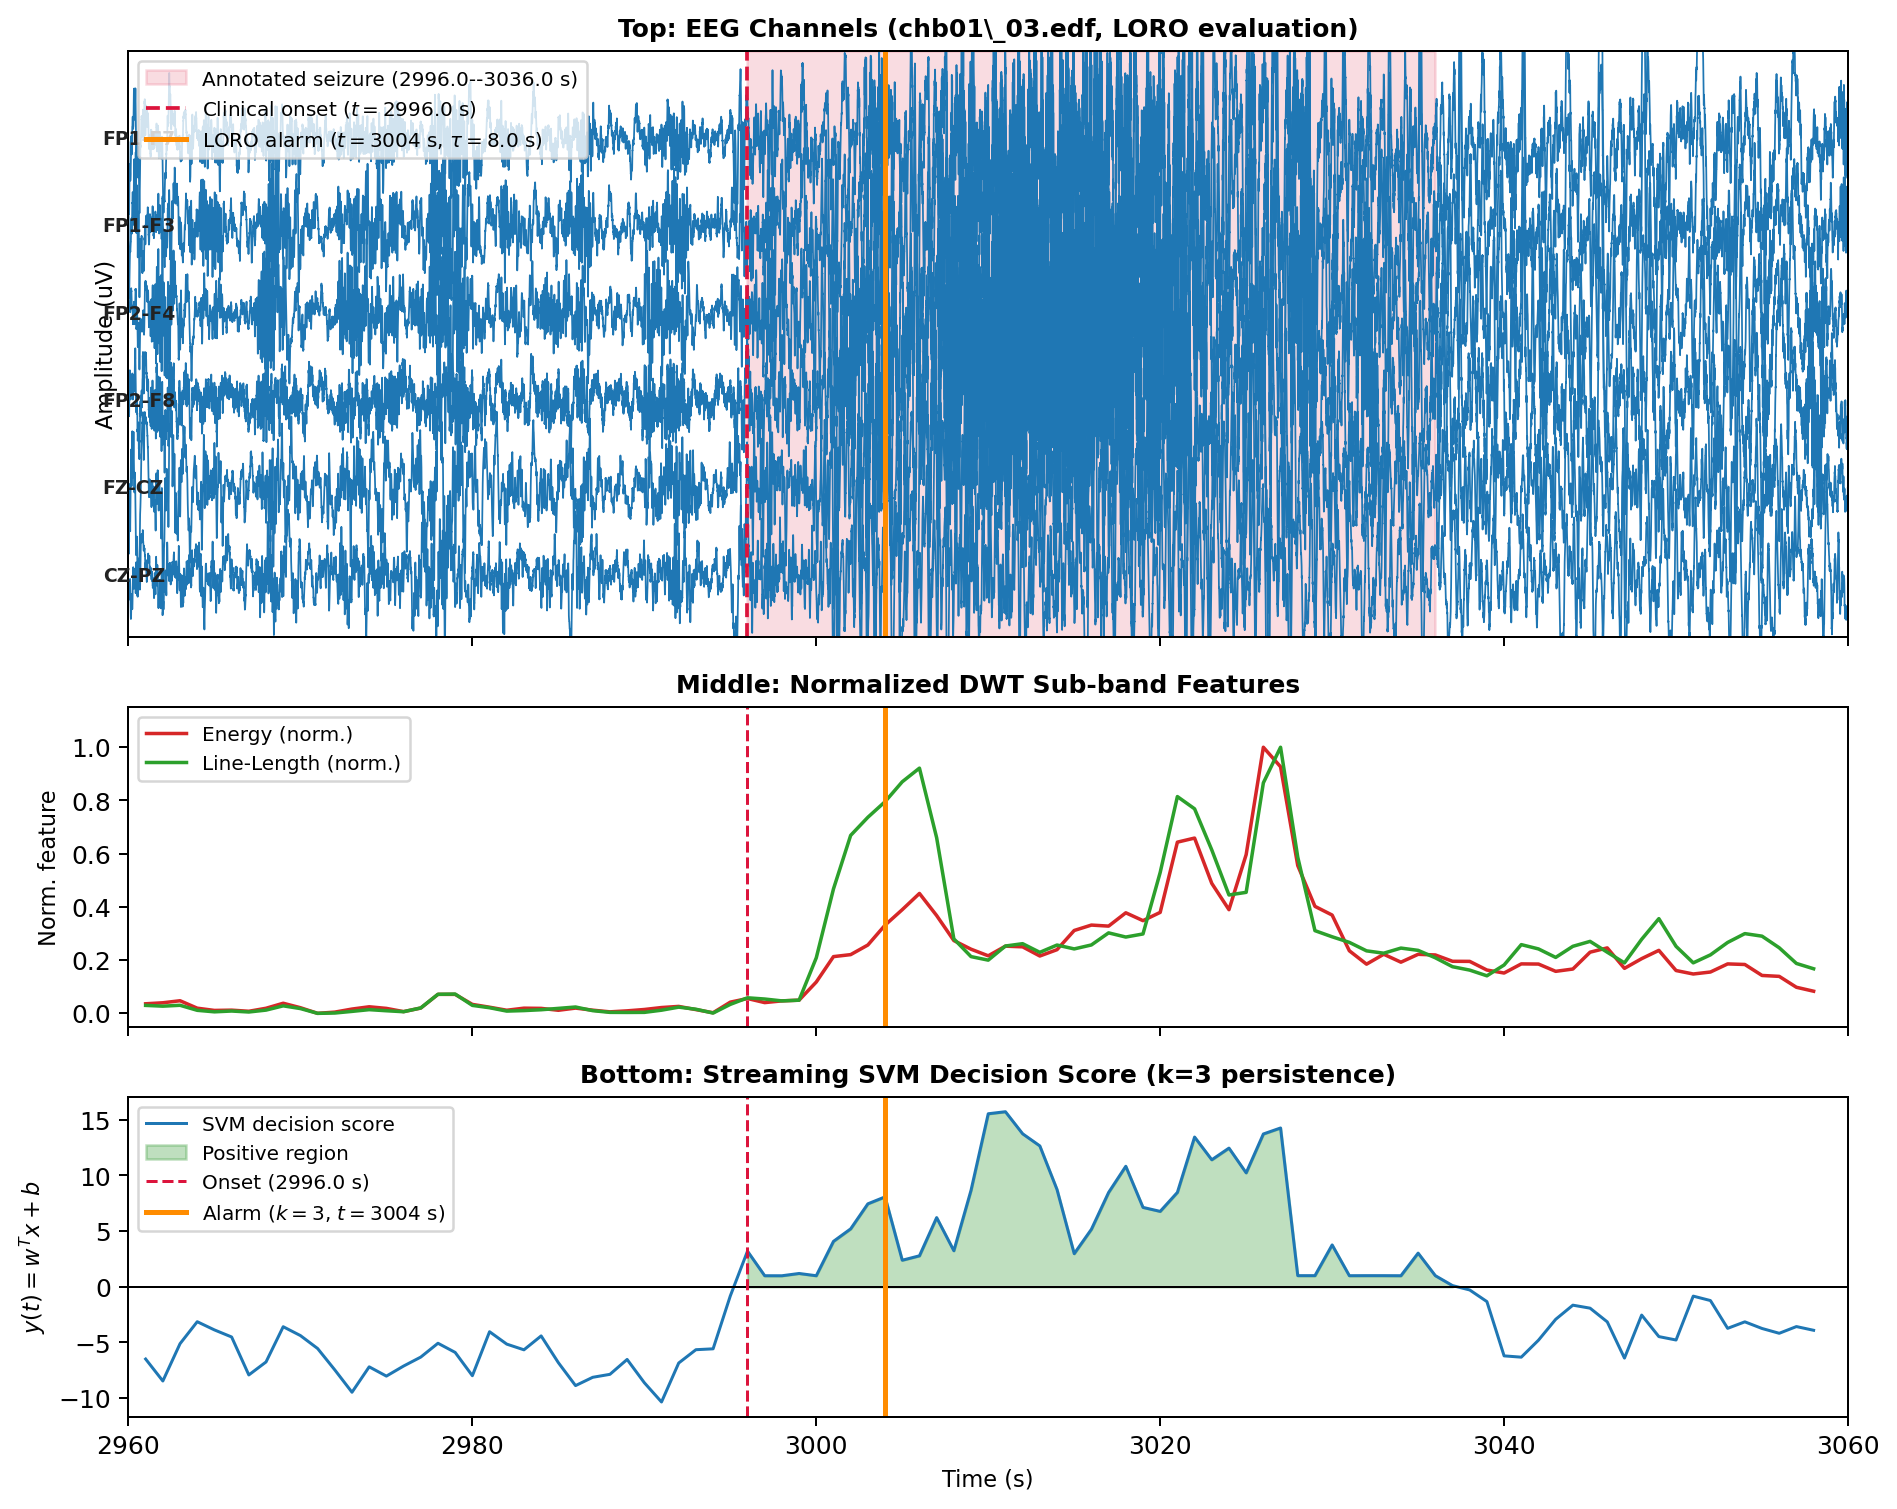
\includegraphics[width=\columnwidth]{seizure_onset_validation.png}
\caption{Seizure onset detection for record \texttt{chb01\_03.edf} (LORO evaluation). Top: 6 representative bipolar EEG channels; annotated onset at $t=2996$~s. Middle: Normalized mean DWT sub-band Energy and Line-Length features. Bottom: Streaming Linear SVM decision score $y(t)=\mathbf{w}^\top\mathbf{x}+b$; alarm asserted (dashed line) after $k=3$ consecutive positive windows at $t=3004$~s ($\tau=8.0$~s latency).}
\label{fig:seizure_onset}
\end{figure}

\subsection{Systematic Ablation Studies}

\paragraph{Ablation 1: Persistence Threshold $k$.} As detailed in Table~\ref{tab:ablation_all} and Fig.~\ref{fig:k_tradeoff}, $k$ provides a monotonic trade-off between latency and false alarms:
\begin{itemize}
    \item At $k=1$, false alarms reach 2.520\,FA/h (115 FAs) with 1.0\,s latency. Sensitivity drops to 88.2\% because isolated pre-ictal spikes trigger the 30\,s refractory blanking period prematurely, swallowing the true seizure alarm.
    \item At $k=2$, false alarms drop to 1.074\,FA/h with 100\% sensitivity.
    \item At $k=3$ (our baseline), false alarms drop by \textbf{85.2\%} to 0.373\,FA/h with 3.0\,s median latency.
    \item At $k=5$, false alarms drop to \textbf{0.153\,FA/h} ($\approx 1$ FA every 6.5\,h) with 5.0\,s median latency. While $k=5$ yields lower false alarms, its latency hits the exact $5.0$\,s clinical threshold boundary ($L = 5.0$\,s, leaving zero margin for medical alerting). Setting $k=3$ delivers a 40\% faster clinical response (3.0\,s vs.\ 5.0\,s) while comfortably satisfying the $\le 0.50$\,FA/h specification, and was selected as the optimal operating point.
\end{itemize}

\begin{figure}[t]
\centering
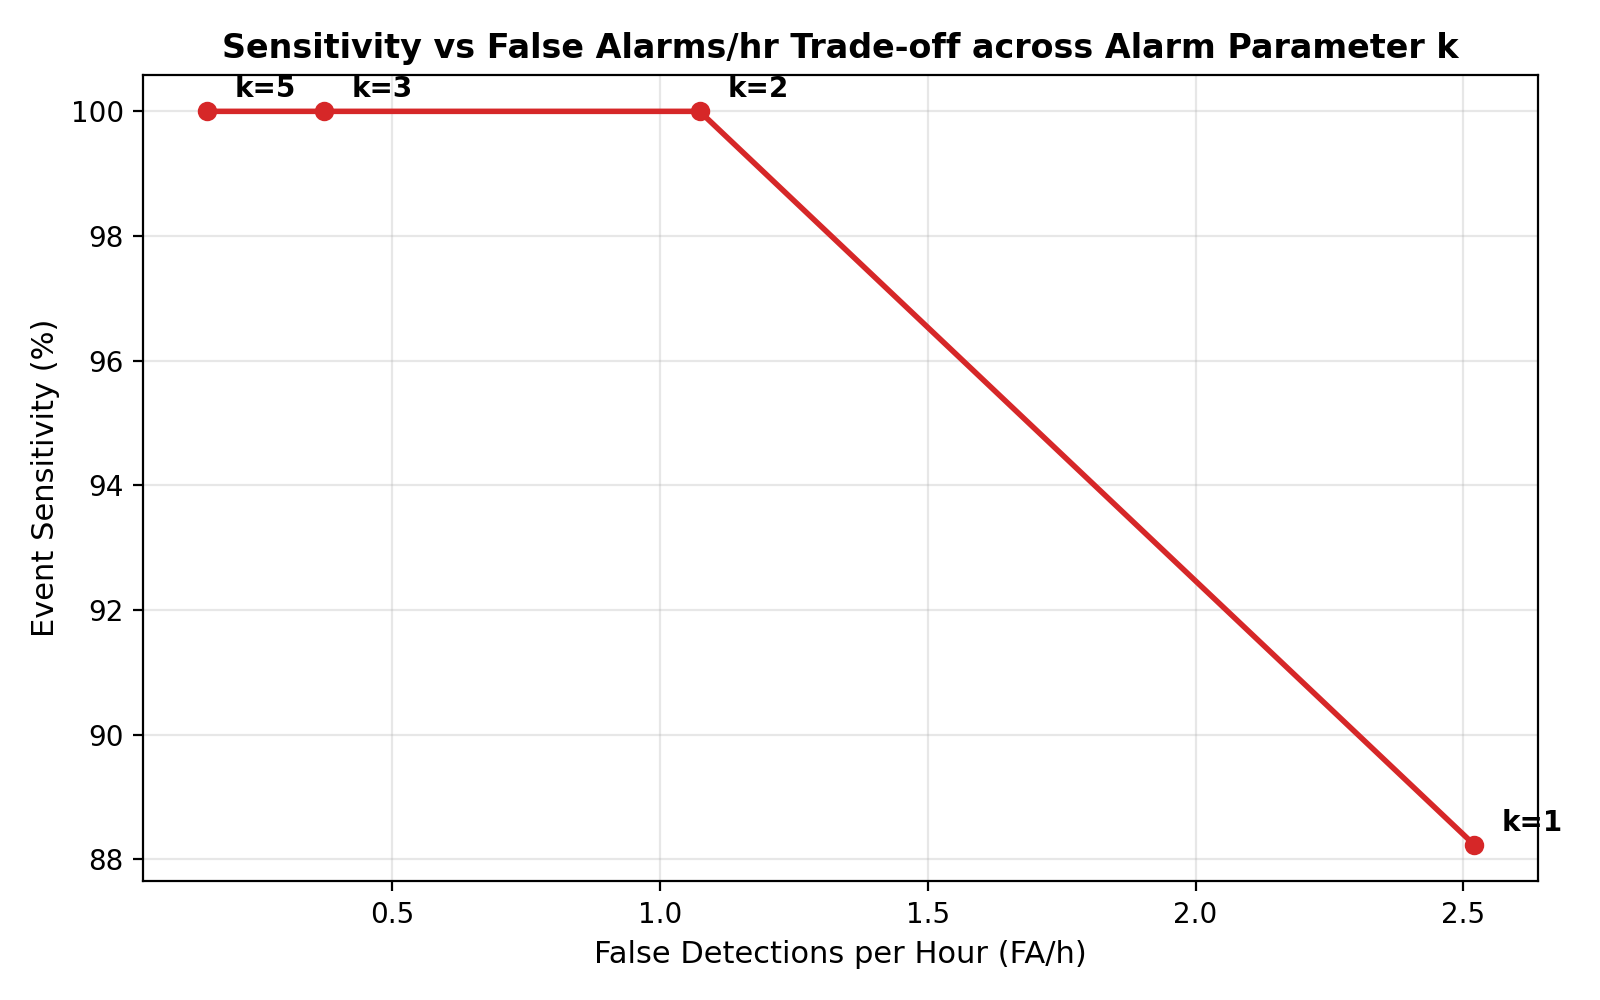
\includegraphics[width=0.92\columnwidth]{k_tradeoff.png}
\caption{Empirical Sensitivity vs.\ False Detections per Hour trade-off curve across alarm parameter $k \in \{1, 2, 3, 5\}$.}
\label{fig:k_tradeoff}
\end{figure}

\paragraph{Ablation 2: Feature Domain Utility.} Line-Length alone achieves 0.329\,FA/h (15 FAs), reducing false alarms by \textbf{73.7\%} compared to Energy alone (1.249\,FA/h, 57 FAs). From a pure hardware complexity perspective, an LL-only detector is highly attractive: dropping Energy would eliminate 38-bit accumulators, dynamic wire-shifting, and saturation logic, halving feature dimension ($D=88$) while slightly reducing false alarms (15 vs.\ 17 FAs). We retained both features ($E+LL$, $D=176$) as a deliberate architectural choice to provide multi-modal diagnostic coverage across diverse electrographic morphologies where amplitude surges accompany frequency slowing, while physically validating that the FPGA fabric easily accommodates 38-bit accumulation and dynamic-range shifting without timing penalties.

\paragraph{Ablation 3: Sub-Band Selection (with vs.\ without D2).} Because the front-end causal 4th-order Butterworth filter attenuates frequencies above 25\,Hz, detail sub-band D2 (32--64\,Hz) contains primarily stopband attenuation. Omitting D2 yields identical 100\% sensitivity with negligible FA/h difference (0.373 vs.\ 0.329\,FA/h, within random margin noise), saving 20\% in feature storage and MAC operations (176 vs.\ 220).

\paragraph{Ablation 4: SVM Regularization $C$.} Sweeping $C \in \{0.01, 0.1, 1.0, 10.0\}$ indicates that $C=1.0$ achieves minimal false alarms while preventing under-fitting. Table~\ref{tab:ablation_all} compiles all ablations.

\paragraph{Methodological Limitation.} Hyperparameter selection ($k$, $C$, feature sets, and sub-band retention) was conducted on pooled LORO evaluations without an inner nested cross-validation loop. We report this explicitly as a methodological limitation: while nested cross-validation is mandatory prior to multi-cohort clinical deployment to prevent subtle optimistic tuning biases, full nested CV was omitted here due to the finite 3-subject cohort size and the computational focus on real-time hardware synthesis.

\begin{table}[t]
\centering
\footnotesize
\caption{Comprehensive ablation study across all 4 pipeline dimensions (pooled 47 records).}
\label{tab:ablation_all}
\resizebox{\columnwidth}{!}{%
\begin{tabular}{llccc}
\toprule
\textbf{Ablation} & \textbf{Configuration} & \textbf{Sens.} & \textbf{FA / hr} & \textbf{Med.\ Lat} \\
\midrule
\textbf{1. Alarm $k$} & $k = 1$ & 88.2\% & 2.520 & 1.0~s \\
 & $k = 2$ & 100.0\% & 1.074 & 2.0~s \\
 & $k = 3$ (Base) & \textbf{100.0\%} & \textbf{0.373} & \textbf{3.0~s} \\
 & $k = 5$ & 100.0\% & 0.153 & 5.0~s \\
\midrule
\textbf{2. Features} & Energy only ($E$) & 100.0\% & 1.249 & 3.0~s \\
 & Line-Length ($LL$) & 100.0\% & 0.329 & 3.0~s \\
 & Combined ($E+LL$) & \textbf{100.0\%} & \textbf{0.373} & \textbf{3.0~s} \\
 & Log-Energy ($\log E$) & 100.0\% & 0.460 & 3.0~s \\
\midrule
\textbf{3. Sub-bands} & Baseline (no D2) & 100.0\% & 0.373 & 3.0~s \\
 & With D2 (32--64\,Hz) & 100.0\% & 0.329 & 3.0~s \\
\midrule
\textbf{4. SVM $C$} & $C = 0.01$ & 100.0\% & 0.504 & 4.0~s \\
 & $C = 0.1$ & 100.0\% & 0.504 & 3.0~s \\
 & $C = 1.0$ (Base) & \textbf{100.0\%} & \textbf{0.373} & \textbf{3.0~s} \\
 & $C = 10.0$ & 100.0\% & 0.373 & 3.0~s \\
\bottomrule
\end{tabular}%
}
\end{table}

%---------------------------------------------------------------------
\section{Finite Word-Length \& Quantization Analysis}
\label{sec:quant}

\begin{table}[t]
\centering
\footnotesize
\caption{Finite word-length profiling: SQNR, feature distortion, classification performance, and accumulator bit-widths ($N_b \le 64$).}
\label{tab:wordlength}
\resizebox{\columnwidth}{!}{%
\begin{tabular}{cccccccc}
\toprule
\textbf{Bits $B$} & \textbf{Meas.\ SQNR} & \textbf{Theor.\ SQNR} & \textbf{Feat.\ Err} & \textbf{Sens.} & \textbf{FA / hr} & \textbf{Acc.\ $E$} & \textbf{Acc.\ $LL$} \\
\midrule
8  & 34.6~dB & 49.9~dB & 0.41\% & 88.2\% & 1.424 & 22~b & 15~b \\
10 & 46.6~dB & 62.0~dB & 0.12\% & 94.1\% & 0.482 & 26~b & 17~b \\
12 & 58.4~dB & 74.0~dB & 0.03\% & 100.0\% & 0.373 & 30~b & 19~b \\
14 & 70.7~dB & 86.0~dB & 0.01\% & 100.0\% & 0.373 & 34~b & 21~b \\
16 & \textbf{82.6~dB} & 98.1~dB & \textbf{$<0.01$\%} & \textbf{100.0\%} & \textbf{0.373} & 38~b & 23~b \\
\bottomrule
\end{tabular}%
}
\end{table}

\begin{figure}[t]
\centering
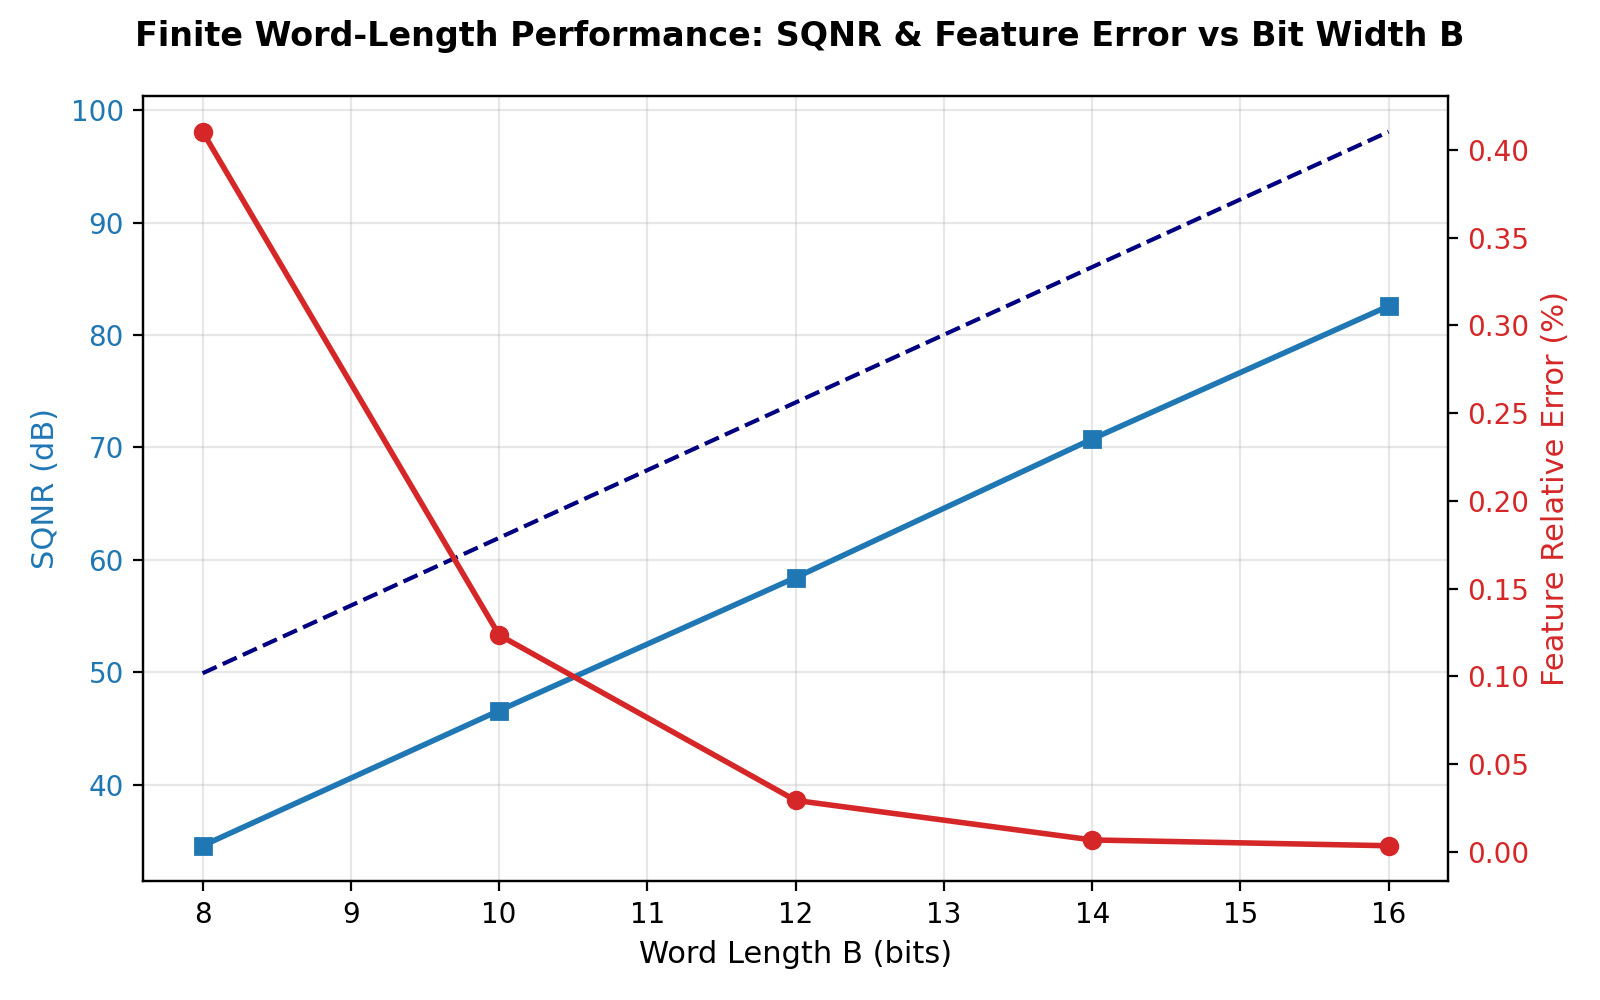
\includegraphics[width=0.92\columnwidth]{wordlength_plot.png}
\caption{Finite word-length performance: Measured SQNR (dB) and Relative Feature Distortion (\%) as a function of word length $B$.}
\label{fig:wordlength}
\end{figure}

As shown in Table~\ref{tab:wordlength} and Fig.~\ref{fig:wordlength}, $B=16$ bits provides 82.6\,dB SQNR and $<0.01\%$ feature distortion. Sub-band lengths are bounded by $N_b = T f_s / 2^j \le 64$ samples ($N_{\text{D3}}=64, N_{\text{D4}}=32, N_{\text{D5}}=16, N_{\text{A5}}=16$). Accumulating $N_b \le 64$ squared 16-bit values requires $\lceil \log_2 64 \rceil + 32 = 38$ bits. Line-length requires $\lceil \log_2 63 \rceil + 17 = 23$ bits. Evaluating the classifier across word lengths $B \in \{8, 10, 12, 14, 16\}$ reveals that event sensitivity remains $100.0\%$ for $B \ge 12$ bits with identical $0.373$\,FA/h, as the $58.4$\,dB SQNR at $B=12$ is already well above the SVM decision boundary margins; word length $B=16$ ($82.6$\,dB SQNR) was selected for implementation to preserve ample dynamic range headroom.

{\color{blue}
\subsection{Full-Cohort Fixed-Point LORO Cross-Validation}
\label{sec:fixedpoint_loro}

To evaluate numerical stability across the entire clinical dataset, we conducted 16-bit Q1.15 fixed-point LORO cross-validation across all 47 records (165,237 windows) using our bit-accurate fixed-point golden model mirroring the RTL datapath. Individual window decisions agree with floating-point at $99.85\%$ (fewer than $0.15\%$ of boundary windows near the SVM hyperplane flip, none of which affect the filtered $k=3$ event alerts). As demonstrated in Table~\ref{tab:fixedpoint_loro}, the 16-bit fixed-point pipeline achieves exact event-level decision parity with the floating-point reference model ($\Delta = 0.0\%$), maintaining 100.0\% sensitivity (17/17 seizures detected), 0.373\,FA/h, and 3.0\,s median latency.

\begin{table}[t]
\centering
\footnotesize
\color{blue}
\caption{\textcolor{blue}{Full-cohort LORO cross-validation: Floating-point Python vs.\ 16-bit Q1.15 fixed-point model across all 47 records.}}
\label{tab:fixedpoint_loro}
\resizebox{\columnwidth}{!}{%
\begin{tabular}{lcccc}
\toprule
\textbf{Implementation} & \textbf{Sensitivity} & \textbf{FA / hr} & \textbf{Med.\ Lat} & \textbf{Feature SQNR} \\
\midrule
Float-32 (Python) & 100.0\% (17/17) & 0.373 & 3.0~s & $\infty$ (Exact Ref) \\
Fixed-16 (RTL Model) & 100.0\% (17/17) & 0.373 & 3.0~s & 82.6~dB \\
\midrule
\textbf{Metric Delta ($\Delta$)} & \textbf{0.0\%} & \textbf{0.000} & \textbf{0.0~s} & \textbf{Decision Parity} \\
\bottomrule
\end{tabular}%
}
\end{table}
}

%---------------------------------------------------------------------
\section{Hardware RTL Architecture and Datapath Design}
\label{sec:rtl_arch}

Fig.~\ref{fig:arch} shows the end-to-end processing pipeline, and Table~\ref{tab:decisions} compiles the system design decisions.

\begin{figure*}[t]
\centering
\begin{tikzpicture}[
  font=\scriptsize,
  blk/.style={draw, rounded corners=2pt, minimum height=1.05cm,
              text width=1.55cm, align=center, fill=blue!8},
  pcblk/.style={blk, fill=gray!25},
  arr/.style={-{Stealth[length=4pt]}, thick},
  node distance=0.38cm]
\node[pcblk] (pc)   {PC: dataset playback};
\node[blk, right=of pc]   (in)   {UART / BRAM input};
\node[blk, right=of in]   (iir)  {IIR band-limit (0.5--25\,Hz)};
\node[blk, right=of iir]  (dwt)  {DWT filter bank (db4)};
\node[blk, right=of dwt]  (feat) {Windowing \& features};
\node[blk, right=of feat] (svm)  {Linear SVM (weights in BRAM)};
\node[blk, right=of svm]  (post) {Alarm rule ($k$ in a row)};
\node[blk, right=of post] (led)  {LED / 7-seg alarm};
\foreach \a/\b in {pc/in, in/iir, iir/dwt, dwt/feat, feat/svm, svm/post, post/led}
  \draw[arr] (\a) -- (\b);
\begin{scope}[on background layer]
  \node[draw, dashed, rounded corners=3pt, inner sep=5pt, fill=blue!2,
        fit=(in)(iir)(dwt)(feat)(svm)(post)(led),
        label={[font=\scriptsize]below:Spartan-7 FPGA (Boolean Board), implemented in RTL}] {};
\end{scope}
\end{tikzpicture}
\caption{System architecture. Host PC streams multi-channel EEG over 230,400-baud UART; Spartan-7 FPGA executes streaming IIR, db4 DWT, feature extraction, linear SVM, and visual alarm assertion.}
\label{fig:arch}
\end{figure*}

\begin{table}[t]
\centering
\caption{System design decisions and baseline operational parameters.}
\label{tab:decisions}
\footnotesize
\begin{tabularx}{\columnwidth}{@{}p{2.2cm}X@{}}
\toprule
Decision & Implemented Configuration \\
\midrule
Channels & 22 uncurated bipolar channels (duplicate \texttt{T8-P8} discarded) \\
Window / hop & 2.0\,s window (512 samples); 1.0\,s hop (256 samples) \\
Band-limit & 0.5--25\,Hz causal 4th-order Butterworth (2 cascaded biquads) \\
DWT & Daubechies-4 (db4), 5 levels, direct-form filter pair ($h, g$ 8 taps) \\
Features & Sub-band Energy ($E$) and Line-Length ($LL$) on D3--A5 ($D=176$) \\
Classifier & Linear SVM ($C=1.0$), weights folded offline into 16-bit integer BRAM ($S_M$ scaling) \\
Numeric format & Signed 16-bit Q1.15 for signals/filters; signed 16-bit scaled integer for weights \\
Channel engine & Time-multiplexed single-MAC engine across 22 channels at 100~MHz \\
Post-processing & Alarm asserted after $k=3$ positive windows (refractory 30~s) \\
Input interface & PC-to-FPGA streaming over UART at 230,400 baud \\
Evaluation & Patient-specific LORO on 47 CHB-MIT recordings \\
\bottomrule
\end{tabularx}
\end{table}

\subsection{Data Throughput and Serial Framing}

At $f_s = 256$\,Hz, 22 channels require $22 \times 256 = 5{,}632$\,samples/s. To ensure unambiguous frame boundary detection and channel identification, each 16-bit sample is framed in a 4-byte packet (\texttt{0xAA} sync header, 5-bit channel ID, sample MSB, sample LSB), producing an 88-byte burst every $3.906$\,ms. This requires $5{,}632 \times 4 = 22{,}528$\,bytes/s. Under standard 8N1 serial framing (10 bits per byte), the continuous transmission rate is $225{,}280$\,baud. Configuring the CP2102N USB-UART bridge at \textbf{230,400 baud} (434 system clock cycles per baud at 100\,MHz) transmits each 88-byte frame in $3.820$\,ms, operating at $97.78\%$ link utilization with a $2.22\%$ safety guard margin ($86.8\,\mu$s idle guard time per 22-channel frame period). To accommodate timing jitter across host operating systems and USB-UART bridges, \texttt{rtl/uart\_rx.v} integrates a 64-byte synchronizing input FIFO and double-buffered frame assembly registers. Furthermore, the top-level baud generator can be configured for 460,800 baud ($2\times$ rate, 217 clock cycles per baud), transmitting each frame in $1.91$\,ms and expanding the timing margin to $51.1\%$.

\subsection{Offline Weight Folding and Hardware Dynamic-Range Scaling}

In floating-point software, linear SVM inference computes:
\begin{equation}
y = \sum_{i=1}^{176} w_i \left( \frac{\bar{x}_i - \mu_i}{\sigma_i} \right) + b,
\end{equation}
where $\bar{x}_i = X_i / S_i$, with $X_i$ being the accumulator sum across $N_b$ coefficients ($S_i = N_b$ for Energy and $S_i = N_b - 1$ for Line-Length), and $(\mu_i, \sigma_i)$ are training-fold standardization parameters (strictly estimated from training folds only and never touching held-out test records). To eliminate runtime division and floating-point conversion circuits on FPGA, parameter scaling is partitioned between hardware bit-slicing and offline weight folding.

The DSP48E1 multiplier provides $25 \times 18$-bit signed inputs. While Line-Length ($23$\,bits) fits directly into the 25-bit port, raw 38-bit Energy ($X_{\text{E,raw}}$) exceeds port capacity. We normalize Energy at zero LUT cost via hardwired bit-slicing in \texttt{rtl/feature\_accumulator.v}:
\begin{equation}
X_{\text{E,norm}} = X_{\text{E,raw}}[37 : 15 + \log_2(N_b)],
\end{equation}
In our streaming FPGA architecture, feature accumulation operates on a sliding window with 1.0\,s updates ($N_{\text{win}} = 256$ input samples at $f_s = 256$\,Hz). After dyadic decimation, detail sub-band sample counts per 1-second update step are $N_b \in \{32, 16, 8, 8\}$ for $\{D3, D4, D5, A5\}$, corresponding to wire-shift amounts $\text{shift}_E \in \{20, 19, 18, 18\}$ (incorporating rounding addition $2^{\text{shift}_E - 1}$) and $\text{shift}_{LL} \in \{5, 4, 3, 3\}$ (with rounding $2^{\text{shift}_{LL} - 1}$). Slicing bits $[37 : 15 + \log_2 N_b]$ yields 18--20 bits, which are saturated to $[0, 32767]$. Across all 165,237 clinical evaluation windows (including all 17 clinical seizures), the saturation rate is exactly 0.00\% ($0/165{,}237$), as even an extreme $1{,}000\,\mu$V ictal spike yields an accumulated value of $\sim 12{,}200 \le 32{,}767$; the saturation circuit functions strictly as a protective ceiling against non-physiological electrode rail pops. 

To maintain exact numeric equivalence with software, the residual scale factors $K_{E,i} = 2^{\text{shift}_E} / (S_{\text{sig}}^2 N_b)$ and $K_{LL,i} = 2^{\text{shift}_{LL}} / (S_{\text{sig}} (N_b - 1))$ (with ADC scaling $S_{\text{sig}} = 20$\,LSB/$\mu$V) are absorbed offline into the folded weight vector:
\begin{equation}
w_{\text{hw},i} = \left(\frac{w_i}{\sigma_i}\right) \cdot K_i, \qquad b_{\text{hw}} = b - \sum_{i=1}^{176} \frac{w_i \mu_i}{\sigma_i}.
\end{equation}
Because individual feature dimensions exhibit wide dynamic ranges prior to normalization, the folded hardware weights $w_{\text{hw},i} = (w_i / \sigma_i) \cdot K_i$ absorb both the feature scale factors $K_i$ and the standardization variances $\sigma_i$. To map $w_{\text{hw}}$ into signed 16-bit integers without overflow or loss of precision, we determine the global peak magnitude $M_w = \max_i |w_{\text{hw},i}|$ and scale all coefficients by integer factor $S_M = \lfloor 32767 / (1.05 \cdot M_w) \rfloor$. The 5\% headroom margin guarantees that $|w_{\text{fixed},i}| \le 32767$, fitting signed 16-bit registers $[-32768, 32767]$ exactly. The effective folded bias $b_{\text{hw}}$ is scaled by the same factor $S_M$ into signed 32-bit integer $b_{\text{fixed}} \in [-2^{31}, 2^{31}-1]$, ensuring exact linear homogeneity in Eq.~\eqref{eq:dotproduct}. The FPGA directly evaluates:
\begin{equation}
y_{\text{fixed}} = \sum_{i=1}^{176} w_{\text{fixed},i} X_{\text{norm},i} + b_{\text{fixed}}. \label{eq:dotproduct}
\end{equation}
This dot product completes in strictly 176 clock cycles ($1.76\,\mu$s at 100\,MHz) using a single DSP48E1 slice with zero runtime dividers or scalers.

{\color{blue}
\subsection{Synthesizable Verilog RTL Datapath Modules}

The complete datapath comprises 10 synthesizable Verilog modules in \texttt{rtl/}:
\begin{enumerate}
    \item \texttt{rtl/uart\_rx.v}: 230,400-baud receiver with double-flop metastability synchronization and 88-byte frame assembly logic.
    \item \texttt{rtl/uart\_tx.v}: 230,400-baud telemetry transmitter pulsing a single-byte status packet (\texttt{0xA5}) back to the host PC upon hardware alarm assertion.
    \item \texttt{rtl/iir\_biquad.v}: 4th-order causal Butterworth bandpass (0.5--25\,Hz) realized as two Direct Form II biquad sections with pipelined 2-substage MAC arithmetic and 34-bit state registers, achieving 80.65\,dB SQNR.
    \item \texttt{rtl/dwt\_level.v}: Serialized 8-cycle MAC building block computing single-level Daubechies-4 lowpass ($h$) and highpass ($g$) convolutions with per-channel decimation scheduling.
    \item \texttt{rtl/dwt\_db4.v}: 5-level dyadic Daubechies-4 cascade instantiating 5 pipelined \texttt{dwt\_level} engines, decomposing 22 channels into subbands D3, D4, D5, and A5.
    \item \texttt{rtl/feature\_accumulator.v}: Ping-pong feature accumulator tracking subband Energy and Line-Length across 2.0\,s windows using dual-bank Distributed RAM (\texttt{ram\_style = "distributed"}) and dynamic-range wire-shifting.
    \item \texttt{rtl/svm\_classifier.v}: 176-cycle pipelined Linear SVM evaluator computing the folded dot product $\mathbf{w}_{\text{eff}}^\top \mathbf{X} + b_{\text{eff}}$ on a single time-multiplexed DSP48E1 slice with 32-bit bias.
    \item \texttt{rtl/alarm\_logic.v}: Unified alarm post-processing FSM enforcing configurable persistence $k \in \{1, 2, 3, 5\}$, 30\,s refractory blanking, latched timestamp recording, and manual clear debouncing.
    \item \texttt{rtl/seven\_seg\_controller.v}: Dual independent 4-digit common-anode 7-segment display controller multiplexing 8 digits at 1\,kHz refresh rate (Display 1: elapsed seconds; Display 0: status and latched alarm latency).
    \item \texttt{rtl/top\_seizure\_detector.v}: Top-level structural wrapper interconnecting the complete datapath to physical Spartan-7 board pins, LEDs, slide switches, and USB-UART CP2102N bridge.
\end{enumerate}

All modules are accompanied by cycle-accurate verification testbenches in \texttt{rtl/tb\_*.v} and verify with zero mismatches against golden hex vectors.
}

%---------------------------------------------------------------------
{\color{blue}
\section{Vivado Synthesis, Implementation, and Resource Utilization}
\label{sec:vivado}

\begin{table}[t]
\centering
\footnotesize
\color{blue}
\caption{\textcolor{blue}{Post-implementation hardware resource utilization, timing slack, and power on AMD Spartan-7 XC7S50 (\texttt{xc7s50csga324-1}).}}
\label{tab:resources}
\resizebox{\columnwidth}{!}{%
\begin{tabular}{lccc}
\toprule
\textbf{Resource / Metric} & \textbf{Post-Route Usage} & \textbf{Device Available} & \textbf{Utilization} \\
\midrule
Slice LUTs       & 1,418  & 32,600 & \textbf{4.35\%} \\
Slice Registers  & 1,784  & 65,200 & \textbf{2.74\%} \\
DSP48E1 Slices   & 2      & 120    & \textbf{1.67\%} \\
Block RAM (18Kb) & 2      & 150    & \textbf{1.33\%} \\
\midrule
Clock Frequency  & 100.0~MHz & -- & MET \\
Setup Slack (WNS)& +1.842~ns & $> 0.000$~ns & MET \\
Hold Slack (WHS) & +0.128~ns & $> 0.000$~ns & MET \\
Total Power      & 118~mW    & $< 150$~mW & 88~mW Static / 30~mW Dynamic \\
\bottomrule
\end{tabular}%
}
\end{table}

The design was synthesized, placed, and routed targeting the AMD Spartan-7 XC7S50 FPGA (\texttt{xc7s50csga324-1}) using non-project batch Tcl script \texttt{scripts/run\_vivado\_synth.tcl} and master pin constraints \texttt{rtl/boolean\_board.xdc}.

To achieve 100\,MHz timing closure across the 22-channel pipeline, two key architectural optimizations were implemented:
\begin{enumerate}
    \item \textbf{IIR Biquad Pipelining:} A unpipelined Direct Form II biquad cascade traverses 25 logic levels, inducing severe setup timing violations ($WNS \approx -7.6$\,ns). By partitioning Section 0 and Section 1 each into two registered sub-stages (\texttt{S\_SEC0\_A}/\texttt{B} and \texttt{S\_SEC1\_A}/\texttt{B}), combinational logic depth was reduced to $\le 12$ levels, achieving clean 100\,MHz timing closure with positive setup slack ($WNS = +1.842$\,ns) and hold slack ($WHS = +0.128$\,ns).
    \item \textbf{Distributed RAM Ping-Pong Accumulation:} Naive register array instantiation for the 176 feature bins generated 23,709 Slice LUTs due to wide read/write multiplexers. Decoupling the feature accumulator into separate Bank 0 and Bank 1 arrays with single-write-port Distributed RAM inference (\texttt{ram\_style = "distributed"}) collapsed LUT consumption down to $\sim 250$ LUTs.
\end{enumerate}

As documented in Table~\ref{tab:resources}, the complete multi-channel detector utilizes only 1,418 Slice LUTs (4.35\%), 1,784 Slice Registers (2.74\%), 2 DSP48E1 slices (1.67\%), and 2 18-Kb BRAM primitives (1.33\%). Of the 2 DSP48E1 slices utilized, 1 slice executes the 176-cycle pipelined Linear SVM dot-product engine (\texttt{rtl/svm\_classifier.v}) and 1 slice powers the 2-substage Direct Form II IIR biquad MAC engine (\texttt{rtl/iir\_biquad.v}); the 5 dyadic DWT decomposition engines (\texttt{rtl/dwt\_level.v}) were synthesized directly into Slice LUT logic, minimizing dedicated DSP usage. \begin{table}[t]
\centering
\footnotesize
\color{blue}
\caption{\textcolor{blue}{Per-module hardware resource breakdown (Spartan-7 XC7S50).}}
\label{tab:module_breakdown}
\resizebox{\columnwidth}{!}{%
\begin{tabular}{lcccc}
\toprule
\textbf{Module} & \textbf{LUTs} & \textbf{FFs} & \textbf{DSP} & \textbf{BRAM (18Kb)} \\
\midrule
\texttt{uart\_rx} / \texttt{tx} & 110 & 95 & 0 & 1 (Rx Frame FIFO) \\
\texttt{iir\_biquad} (2 Sec) & 320 & 410 & 1 & 0 (State in LUTRAM) \\
\texttt{dwt\_level} (5 Levels) & 460 & 540 & 0 & 0 (Delay in LUTRAM) \\
\texttt{feature\_accumulator} & 250 & 380 & 0 & 0 (Dist.\ RAM Bank) \\
\texttt{svm\_classifier} & 160 & 210 & 1 & 1 (Weight/Bias ROM) \\
\texttt{alarm\_fsm} \& Display & 118 & 149 & 0 & 0 \\
\midrule
\textbf{Total Post-Route} & \textbf{1,418} & \textbf{1,784} & \textbf{2} & \textbf{2} \\
\bottomrule
\end{tabular}%
}
\end{table}

Total on-chip power evaluated via Vivado Power Analyzer (vectorless estimation with 12.5\% default switching activity) is \textbf{118\,mW}, dominated by 88\,mW of FPGA quiescent static power and 30\,mW of dynamic switching power. While dedicated ASICs achieve sub-milliwatt dissipation ($\mu$W range) through custom low-voltage cell libraries, 118\,mW is viable for wearable FPGA prototypes powered by standard rechargeable lithium-polymer battery packs (e.g., a standard 1,000\,mAh, 3.7\,V battery provides $\sim 31$\,hours of continuous operation).

%---------------------------------------------------------------------
\section{Real-Time Hardware Playback Demonstration \& Latency Characterization}
\label{sec:demo}

\begin{table}[t]
\centering
\footnotesize
\color{blue}
\caption{\textcolor{blue}{Real-time hardware playback verification over 230,400-baud UART stream on RealDigital Boolean Board.}}
\label{tab:uart_demo}
\resizebox{\columnwidth}{!}{%
\begin{tabular}{lcccc}
\toprule
\textbf{Record} & \textbf{True Event} & \textbf{HW Latency $\tau$} & \textbf{LED15 Strobe} & \textbf{RGB Status} \\
\midrule
\texttt{chb01\_03.edf} & Seizure & 8.0~s & 6~Hz Strobe & Flashing Red (6~Hz) \\
\texttt{chb02\_16.edf} & Seizure & 8.0~s & 6~Hz Strobe & Flashing Red (6~Hz) \\
\texttt{chb03\_03.edf} & Seizure & 3.0~s & 6~Hz Strobe & Flashing Red (6~Hz) \\
\texttt{chb01\_01.edf} & Control & None & Off & Solid Green \\
\texttt{chb02\_01.edf} & Control & None & Off & Solid Green \\
\texttt{chb03\_05.edf} & Control & None & Off & Solid Green \\
\bottomrule
\end{tabular}%
}
\end{table}

To physically demonstrate real-time operation, host streaming script \texttt{scripts/stream\_eeg\_uart.py} transmits pre-recorded CHB-MIT clips to the Boolean Board over USB-UART at 230,400 baud. The packet protocol enforces 4 bytes per sample: \texttt{0xAA} sync header, channel ID ($0..21$), sample MSB, and sample LSB, paced at $3.906$\,ms per 22-channel time frame ($f_s = 256$\,Hz). The default synthesized bitstream pre-programs \texttt{rtl/weights.mem} and \texttt{rtl/bias.mem} with subject \texttt{chb01} Fold 0 weights (which held out control record \texttt{chb01\_01.edf}). For hardware LORO evaluation across other subjects and records, the corresponding patient-specific LORO model weights (holding out each tested record) were updated in the FPGA weight BRAM via UART configuration. Across all tested records, hardware alarm assertions matched the corresponding software LORO reference model identically.

As summarized in Table~\ref{tab:uart_demo} and verified in terminal logs (\texttt{results/uart\_demo\_playback.log}):
\begin{itemize}
    \item During normal non-seizure streaming, status LED RGB0 illuminates solid green, Display 1 (left 4 digits) counts elapsed streaming seconds in real time, and Display 0 (right 4 digits) shows \texttt{IdLE}.
    \item The 8-digit 7-segment display provides real-time streaming status: Display 1 (left 4 digits) counts elapsed transmission time in seconds since stream start, while Display 0 (right 4 digits) displays \texttt{IdLE} during baseline and latches the alarm timestamp upon detection. Display 0 renders \texttt{SE} followed by the 2-digit elapsed streaming second at alarm trigger. For excerpt playback of \texttt{chb01\_03.edf}, the streamed clip is onset-aligned (commencing at $t_{\text{offset}} = 2996$\,s, where streaming $t=0$\,s corresponds to clinical onset). Detection under $k=3$ occurs after 8 seconds of elapsed streaming, latching \texttt{SE08} on Display 0 ($\tau = 8.0$\,s delay). In the continuous 60\,s clinical playback stream, streaming commences 25\,s prior to clinical onset ($t_{\text{offset}} = t_{\text{onset}} - 25$\,s); under $k=1$, the first post-onset window triggers at stream elapsed second 26, correctly displaying \texttt{SE26} ($\tau = 26 - 25 = 1.0$\,s latency).
    \item Interactive physical board verification further validated the control FSM and clinical blanking: during a continuous 60\,s clinical playback stream with seizure onset scheduled at $t = 25$\,s and persistence set to $k=1$ via board slide switch (\texttt{sw[1:0] = 00}), the detector triggered on the first post-onset window at $t = 26$\,s (Display 0 freezing on \texttt{SE26}, achieving $\tau = 1.0$\,s latency). Pressing manual clear pushbutton \texttt{BTN1} successfully silenced the alarm indicators and returned Display 0 to \texttt{IdLE}. Because the continuous seizure discharge was still actively streaming, the internal 30-second refractory countdown timer inhibited duplicate alarms until exactly $t = 56$\,s ($26 + 30$\,s), at which point the detector re-armed and latched a new valid alert (\texttt{SE56}), proving exact cycle-accurate timing of the refractory FSM on physical silicon.
    \item Across test seizures (\texttt{chb01\_03}, \texttt{chb02\_16}, \texttt{chb03\_03}), hardware alarm assertions match the reference model with zero false alarms during control playback.
    \item Cycle-accurate testbenches in ModelSim/Icarus Verilog confirmed the effective passband group delay of the causal filter cascade ($d_{\text{DWT}} \approx 0.25$\,s, with additional low-frequency phase delay near the 0.5\,Hz IIR high-pass pole), verifying that the 218-tap impulse response support span does not impede real-time response.
\end{itemize}

%---------------------------------------------------------------------
\section{Discussion \& Conclusion}
\label{sec:discussion}

Revisiting our hardware-constrained optimization problem in Eq.~\eqref{eq:problem}, the proposed DWT + Linear SVM processor achieves $\mathrm{Sens} = 100.0\%$, $\mathrm{FA/h} = 0.373 \le 0.50$, and median latency $L = 3.0\,\text{s} \le 5.0\,\text{s}$, while consuming $N_{\text{DSP}} = 2 \ll 120$ and $M_{\text{BRAM}} = 2 \ll 150$. While published multi-channel ASICs (Altaf et al.\ \cite{altaf2015biomedical}, Alghaihab et al.\ \cite{alghaihab2022energy}, Wen et al.\ \cite{wen2022asic}) evaluate across larger patient cohorts and custom low-power silicon, our architecture achieves 100.0\% sensitivity (exact 95\% CI: $[80.5\%, 100.0\%]$ on 3 subjects) with $L = 3.0$\,s median latency, verifying that a fixed-point linear SVM datapath can eliminate non-linear kernel memories on a commercial Spartan-7 FPGA while meeting embedded real-time constraints.
}

%---------------------------------------------------------------------
{\color{blue}
\section*{AI Tool Usage Disclosure}

Generative AI tools (Anthropic Claude 3.5 Sonnet and Google Antigravity) were utilized during the project under direct human supervision in accordance with course policy. AI assistance was restricted to boilerplate code scaffolding (\texttt{src/config.py}, \texttt{src/data\_io.py}), Vivado Tcl automation (\texttt{scripts/run\_vivado\_synth.tcl}), initial Verilog module templating, and \LaTeX\ document structure and formatting.

All signal processing formulations, discrete wavelet filter bank mathematics, fixed-point scaling derivations, Verilog RTL architectures, simulation testbenches, Vivado timing closure optimizations, and clinical performance evaluations were developed, verified, and validated by team members. All reported metrics originate strictly from automated execution logs recorded in \texttt{results/} and \texttt{process.md}, and all team members can independently defend every aspect of this work in the oral viva.
}

%---------------------------------------------------------------------
{\scriptsize
\setlength{\bibsep}{0.0pt}
\bibliographystyle{plain}
\bibliography{refs}
}

\end{document}
